The product we want to create is an intelligent sensor.
This sensor will allow for a new kind of programming that aims to be more intuitive and faster than current methods.
We propose a tool which can be attached to and interface with an existing welding robot. 
By using a special pen to mark the places an object should be welded this sensor can follow the markings to program the robot automatically.
We want to combine the use of computer vision and lasers to determine the localization of the object and the welds.
We want to let the workers change settings via a touch interface so the robot knows how to handle the markings. 

The detection requires a two part localization. 
From a position or set of positions which provide an overview of the object, the sensor will be able to see all markings.
The robot should be able to determine where the markings are on the object. 
This is what we refer to as global localization.

We use a camera and computer vision to locate and move the robot closer to the markings.
The sensor will pick the first marking it can find and move towards that. 
When a marking is found we need to locate the gap between two objects. 
When a gap exist within a marked area it is treated as a place that should be welded.
By using lasers we can determine where there is a gap, as well as determine the angles between the objects.
This part is called local localization.
When a weld is completed the robot will resume searching for markings until there are non left.

We imagine the sensor is mounted on the welding tool as shown in figure \ref{concept_cad}. 
The communication should be done with the robots communication bus to avoid having cables along the robot arm that restrict the mobility.

\begin{figure}[h]
\begin{subfigure}[b]{0.3\textwidth}
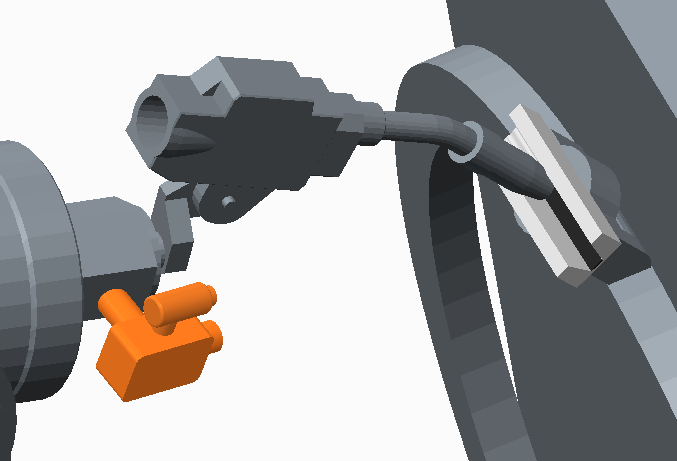
\includegraphics[width=\textwidth]{graphics/CAD1}
\end{subfigure}
\hfill
\begin{subfigure}[b]{0.3\textwidth}
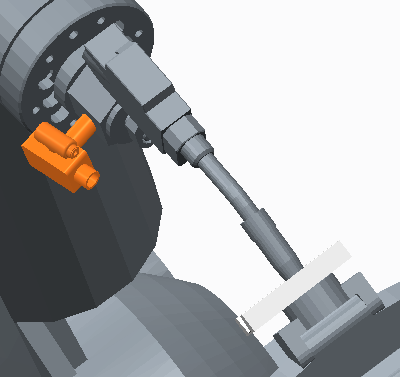
\includegraphics[width=\textwidth]{graphics/CAD2}
\end{subfigure}
\hfill
\begin{subfigure}[b]{0.3\textwidth}
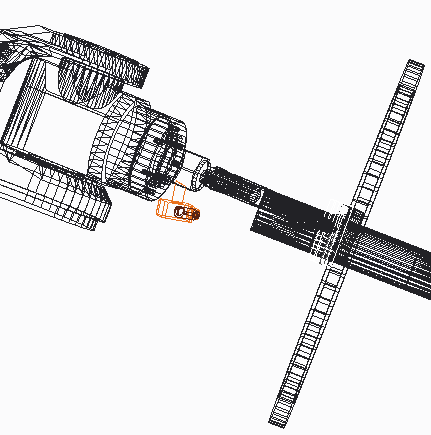
\includegraphics[width=\textwidth]{graphics/CAD3}
\end{subfigure}
\caption{Concept art of the our sensor mounted on a welding robot}
\label{concept_cad}
\end{figure}